\documentclass[11pt]{beamer}

\usepackage[utf8]{inputenc}
\usepackage[french]{babel}
\usepackage{amsmath, amsfonts, amssymb}
\usepackage{csvsimple}
\usepackage{hyperref}
\usepackage[french,boxed,ruled,lined ]{algorithm2e}
\usepackage{graphicx}
\usepackage{tikz}
\usepackage{geometry}

\SetKwFor{Tq}{Tant que}{faire}{FinTantque}
\SetKw{In}{\textbf{Entrées} : }
\SetAlFnt{\small}

\title{Projet de Graph Mining : Diffusion et maximisation d'influence sur les réseaux sociaux}
\author{Nicolas Noblot}
\date{\today}

\setbeamertemplate{footline}[frame number]

\begin{document}
	
	\begin{frame}
		\titlepage
	\end{frame}

	\begin{frame}
		\frametitle{Introduction}
		\begin{itemize}
			\item Réseau social = moyen efficace de diffuser de l'information
			\item Maximisation d'influence  = identifier les noeuds d'un réseau qui contribuent le plus à la diffusion de l'information
			\item \'Etude de diffusion de l'information et de maximisation d'influence sur Facebook et LastFM Asia
			\item Plan : 
			\begin{enumerate}
				\item Rappels théoriques
				\item Présentation des datasets
				\item Résultats et discussion
			\end{enumerate}
		\end{itemize}
	\end{frame}

	\begin{frame}
		\frametitle{Notations}
		\begin{itemize}
			\item{Soit $\mathcal{G} = (V,E)$, si $v\in V$, on note $\mathcal{N}(v)$ l'ensemble des voisins de $v$.}
			\item $\mathcal{S}$ : ensemble des graines, noeuds infectés au départ
			\item $I_t(\mathcal{S})$: ensemble des noeuds infectés à l'instant $t$ dans un processus de diffusion à partir de $\mathcal{S}$
			\item $I(\mathcal{S}) = \bigcup_{t \geq 0} I_t(\mathcal{S})$ :  ensemble des noeuds infectés durant un processus de diffusion à partir de $\mathcal{S}$
			\item{$\mathfrak{S}(\mathcal{S}) = \mathbb{E}(|I(\mathcal{S})|)$ :  espérance du nombre de noeuds infectés à partir de $\mathcal{S}$}
		\end{itemize}
	\end{frame}

	\begin{frame}
		\frametitle{Modèle à cascades indépendantes}
		\begin{columns}
		\begin{column}[c]{0.5\textwidth}
		\resizebox{!}{0.45\textheight}{
		\begin{algorithm}[H]
			\In{$\mathcal{G} = (V, E)$, $\mathcal{S}$}\\
			$I(\mathcal{S})\leftarrow \mathcal{S}$, 
			$\mathcal{A} \leftarrow \mathcal{S}$ \\
			\Tq{$\mathcal{A} \neq \varnothing$}
			{	
				$L \leftarrow \varnothing$ \\
				\PourCh{$a \in \mathcal{A}$}
				{
					\PourCh{$v \in \mathcal{N}(a)$}{
						Choisir un nombre aléatoire $p$ selon $\mathcal{U}\left(\left[0,1\right]\right)$\\
						\eSi{$p < \frac{1}{\text{deg}(v)}$}
						{
							$L\leftarrow L \cup \{v\}$				
						}{
							Ne rien faire
						}
					}
				}
				$\mathcal{A} \leftarrow L \backslash I(\mathcal{S})$ \\
				$I(\mathcal{S}) \leftarrow I(\mathcal{S}) \cup \mathcal{A}$
			}
			\caption{Algorithme de diffusion par cascades}
		\end{algorithm}}
		\end{column}
		\begin{column}[c]{0.35\textwidth}
			\begin{figure}
			\resizebox{!}{0.55\textheight}{
			\begin{tikzpicture}
				\node[draw, circle] (v11) at (0,1) {$v_1$};
				\node[draw, circle] (v21) at (0,2) {$v_2$};
				\node[draw, circle] (v31) at (1,3) {$v_3$};
				\node[draw, circle, fill=red!70] (v41) at (1,1) {$v_4$};
				\node at (-0.7,1) { $\frac{1}{3}$};
				\node at (-0.7,2) {$\frac{1}{3}$};
				\node at (0.3,3) {$\frac{1}{3}$};
				\draw (v41) -- (v31);
				\draw (v41) -- (v21);
				\draw (v41) -- (v11);
				\draw[->, line width=2] (0.5,0) -- (0.5,-1.5);
				\node[draw, circle, fill=red!70] (v12) at (0,-4) {$v_1$};
				\node[draw, circle, fill=black, text=white] (v22) at (0,-3) {$v_2$};
				\node[draw, circle, fill=red!70] (v32) at (1,-2) {$v_3$};
				\node[draw, circle, fill=red!70] (v42) at (1,-4) {$v_4$};
				\draw (v42) -- (v32);
				\draw (v42) -- (v22);
				\draw (v42) -- (v12);
			\end{tikzpicture}}
			\caption{Exemple de cascade. En rouge, les noeuds infectés . En noir, les noeuds sains.}
		\end{figure}
		\end{column}
		\end{columns}
	\end{frame}

	\begin{frame}
		\frametitle{Modèle de seuillage}
		\begin{columns}
		\begin{column}[c]{0.5\textwidth}
			\resizebox{!}{0.45\textheight}{
		\begin{algorithm}[H]
			\caption{Algorithme de diffusion par seuillage}
			\In{$\mathcal{G} = (V, E)$, $\mathcal{S}$} \\
			Initialiser un vecteur $\theta$ de seuils aléatoires entre $0$ et $1$ \\
			$I(\mathcal{S})\leftarrow \mathcal{S}$, 
			$\mathcal{A} \leftarrow \mathcal{S}$ \\
			\Tq{$\mathcal{A} \neq \varnothing$}
			{	
				$L \leftarrow \varnothing$ \\
				\PourCh{$a \in \mathcal{A}$}
				{
					\PourCh{$v \in \mathcal{N}(a)$}{
						Calculer la proportion $p$ de voisins de $v$ infectés\\
						\eSi{$p > \theta_v$}
						{
							$L\leftarrow L \cup \{v\}$				
						}{
							Ne rien faire
						}
					}
				}
				$\mathcal{A} \leftarrow L \backslash I(\mathcal{S})$ \\
				$I(\mathcal{S}) \leftarrow I(\mathcal{S}) \cup \mathcal{A}$
			}				
		\end{algorithm}}
		\end{column}
		\begin{column}[c]{3cm}
			\begin{figure}
				\resizebox{!}{0.55\textheight}{
					\begin{tikzpicture}
						\node[draw, circle] (v11) at (0,1) {$v_1$};
						\node[draw, circle] (v21) at (0,2) {$v_2$};
						\node[draw, circle] (v31) at (1,3) {$v_3$};
						\node[draw, circle, fill=red!70] (v41) at (1,1) {$v_4$};
						\node at (-1.3,1) { $\theta_{v_1} = 0.3$};
						\node at (-0.3,2.7) {$\theta_{v_2} = 0.2$};
						\node at (1,3.8) {$\theta_{v_3} = 0.7$};					
						\draw (v41) -- (v31);
						\draw (v41) -- (v21);
						\draw (v41) -- (v11);
						\draw[->, line width=2] (0.5,0) -- (0.5,-1.5);
						\node[draw, circle, fill=red!70] (v12) at (0,-4) {$v_1$};
						\node[draw, circle, fill=red!70] (v22) at (0,-3) {$v_2$};
						\node[draw, circle, fill=red!70] (v32) at (1,-2) {$v_3$};
						\node[draw, circle, fill=red!70] (v42) at (1,-4) {$v_4$};
						\draw (v42) -- (v32);
						\draw (v42) -- (v22);
						\draw (v42) -- (v12);
				\end{tikzpicture}}
				\caption{\small Exemple d'exécution du modèle de seuillage. Les noeuds infectés sont en rouge.}
			\end{figure}
		\end{column}
	\end{columns}
	\end{frame}
		
	\begin{frame}
		\frametitle{Heuristique gloutonne de maximisation de l'influence}
		\begin{algorithm}[H]
			\In{$\mathcal{G}(V, E)$, budget k} \\
			$\mathcal{S} \leftarrow \varnothing$ \\
			\Tq{$|\mathcal{S}| \leq k$}
			{
				$v^* = \text{argmax}_{v \in V \backslash \mathcal{S}}\left(\mathfrak{S}(\mathcal{S} \cup \{v\})\right) - \mathfrak{S}{S}$\\
				$\mathcal{S} \leftarrow \mathcal{S} \cup \{v^*\}$
			}
			\caption{Heuristique gourmande de maximisation d'influence}
			
		\end{algorithm}
	\vskip 2mm
		\begin{itemize}
			\item Algorithme très calculatoire en pratique.
			\item Estimation de $\mathfrak{S}(\mathcal{S})$ à l'aide de la moyenne empirique du nombre de noeuds infectés sur plusieurs exécutions d'un algorithme de diffusion.
		\end{itemize}
	\end{frame}

	\begin{frame}
	\frametitle{Dataset ego-Facebook}
	\begin{itemize}
		\item Dataset de cercle d'amis sur Facebook
		\item Les noeuds sont les utilisateurs. Un sommet $A$ est relié à un sommet $B$ si $A$ est ami avec $B$.
		\item Graphe non-pondéré et non-orienté
		\item{Statistiques générales :
			\begin{center}
			\csvautotabular{../../data/ego_facebook/facebook/general_stats.csv}
			\end{center}
		} 
		\item \small Source : \href{http://i.stanford.edu/~julian/pdfs/nips2012.pdf}{J. McAuley and J. Leskovec. Learning to Discover Social Circles in Ego Networks. NIPS, 2012.}
	\end{itemize}		
	\end{frame}
	
	\begin{frame}
		\frametitle{Dataset LastFM Asia}
		\begin{itemize}
			\item{Graphe d'utilisateurs en Asie du site LastFM (site de recommandation de musiques)}
			\item{Les noeuds sont les utilisateurs et une arête existe entre $A$ et $B$ s'ils se suivent mutuellement.}
			
			\item{Graphe non-pondéré et non-orienté}
			\item{Statistiques générales : 
				
				\begin{center}
					\csvautotabular{../../data/lastfm_asia/general_stats.csv}
				\end{center}
			}
			\item \small Source : \href{https://arxiv.org/abs/2005.07959}{B. Rozemberczki and R. Sarkar. Characteristic Functions on Graphs: Birds of a Feather, from Statistical Descriptors to Parametric Models. 2020.}
		\end{itemize}
	\end{frame}
	\begin{frame}
		\frametitle{Expériences}
		Sur chaque dataset:
		\begin{itemize}
			\item Maximisation d'influence avec un budget inférieur à 30 noeuds
			\item Utilisation des modèles de seuillage et de cascade avec 6 stratégies de sélection des noeuds de départ différentes : aléatoire, centralité pagerank, centralité closeness, centralité spectrale, centralité intermédiaire, degré
			\item Comparaison avec l'heuristique gourmande 
		\end{itemize}
	\end{frame}
	\begin{frame}
		\frametitle{Résultats de la diffusion sur le dataset Facebook (1/2)}
			\begin{figure}
				\centering
				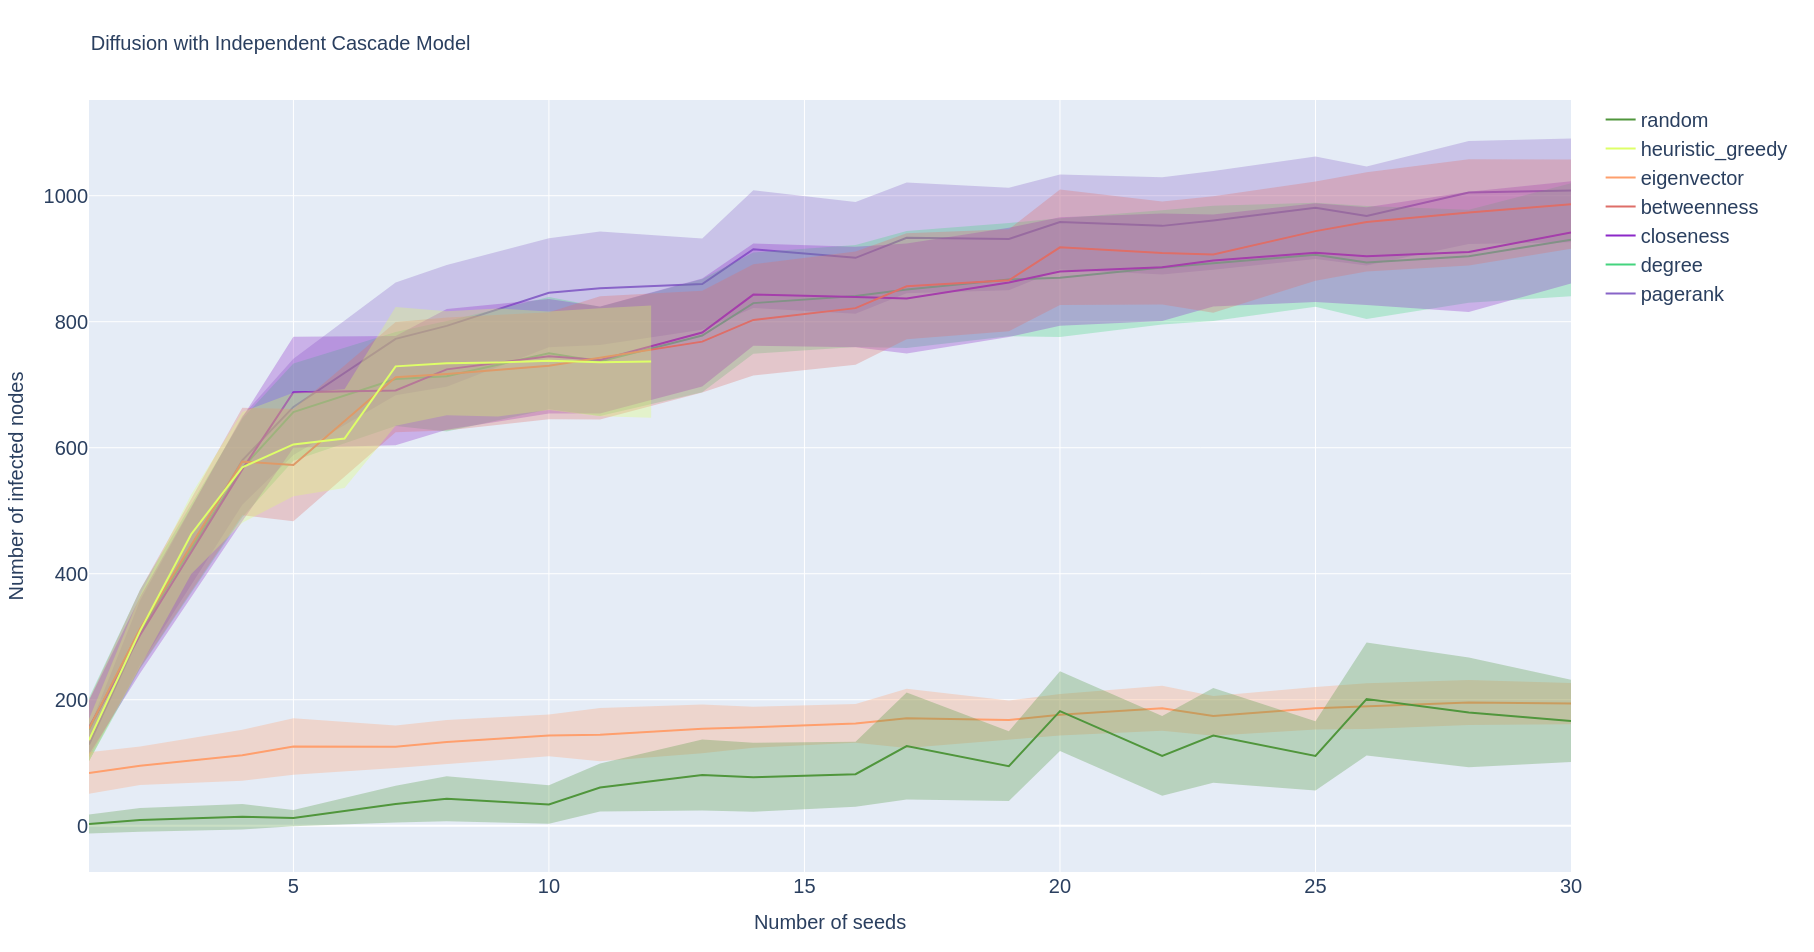
\includegraphics[width=\textwidth, height=0.8\textheight]{./images/facebook_icm.png}
			\end{figure}
	\end{frame}
	\begin{frame}
		\frametitle{Résultats de la diffusion sur le dataset Facebook (2/2)}
		\begin{figure}
			\centering
			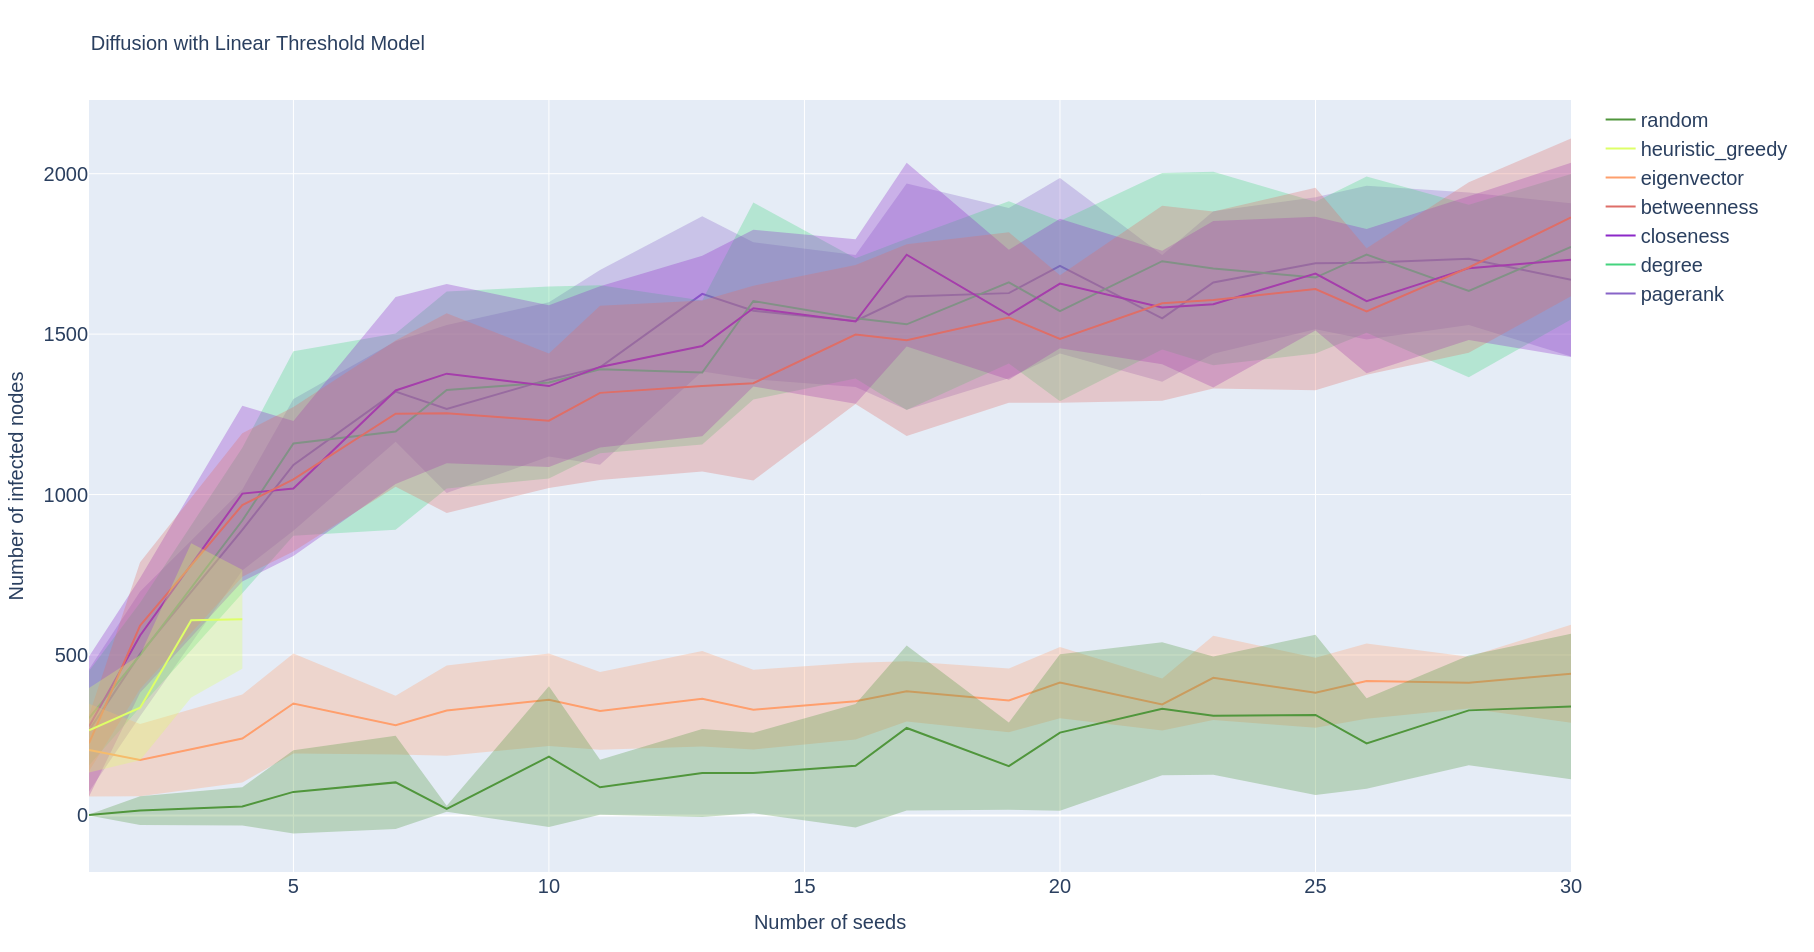
\includegraphics[width=\textwidth, height=0.8\textheight]{./images/facebook_ltm.png}
		\end{figure}
	\end{frame}
	\begin{frame}
		\frametitle{Résultats de la diffusion sur le dataset LastFM Asia (1/2)}
		\begin{figure}
			\centering
			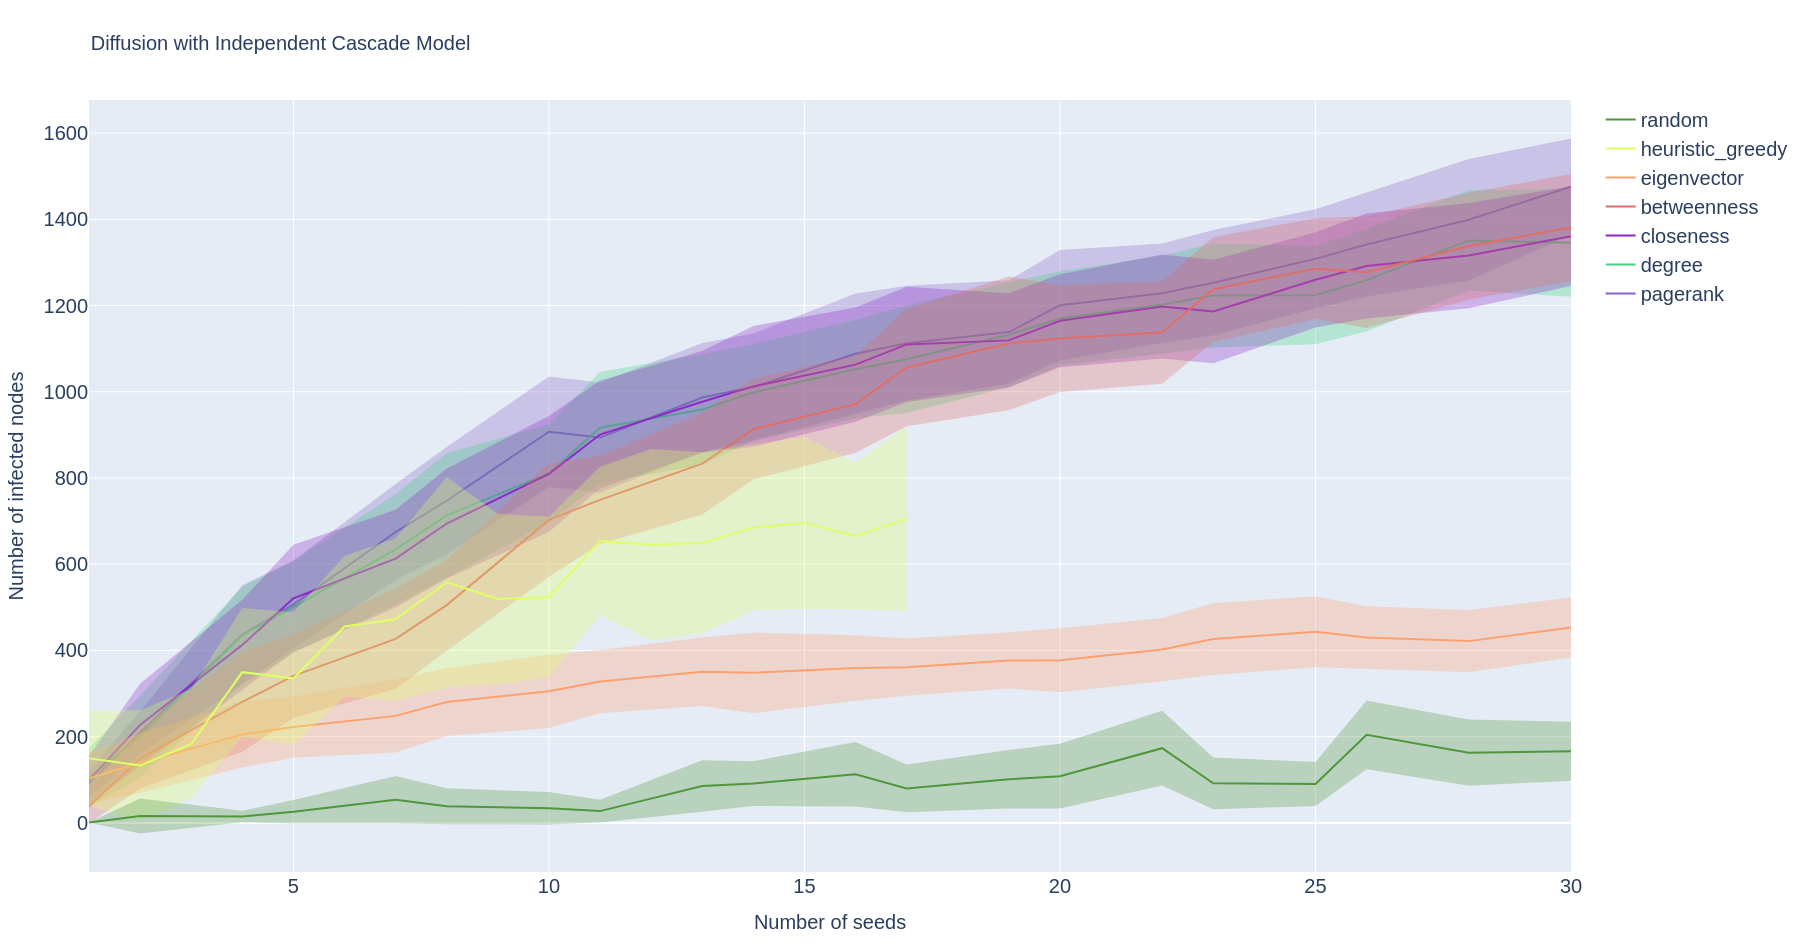
\includegraphics[width=\textwidth, height=0.8\textheight]{./images/lastfm_icm.png}
		\end{figure}
	\end{frame}
	\begin{frame}
		\frametitle{Résultats de la diffusion sur le dataset LastFM Asia (2/2)}
		\begin{figure}
			\centering
			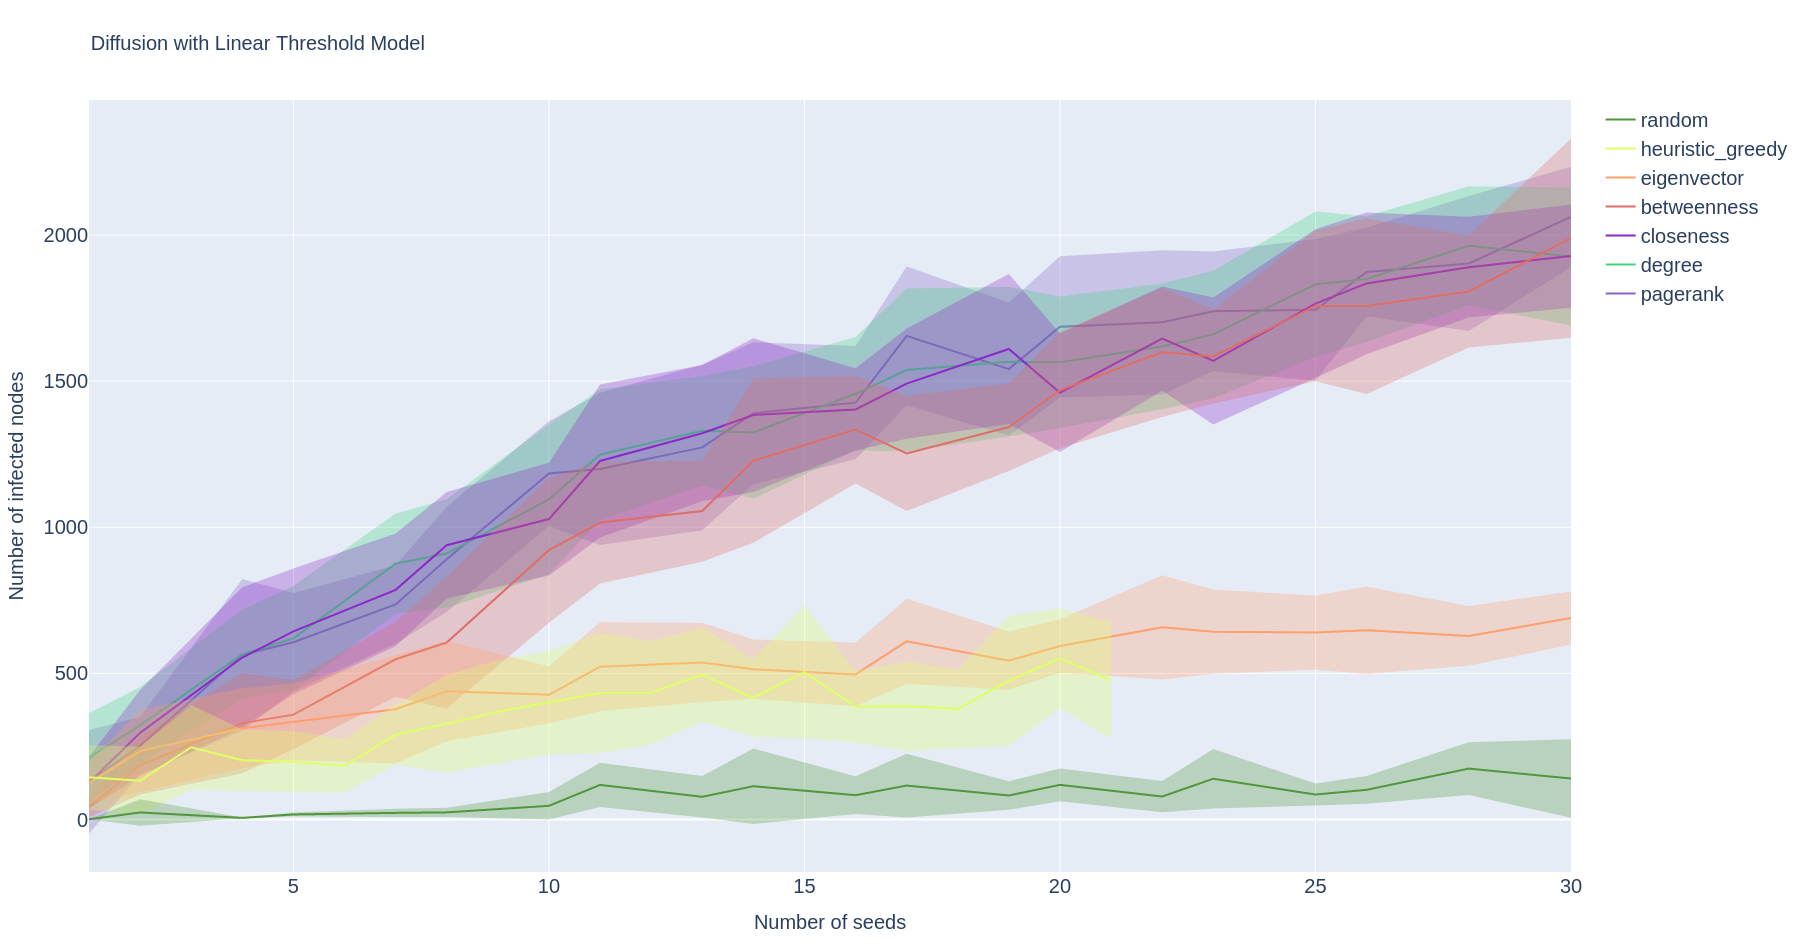
\includegraphics[width=\textwidth, height=0.8\textheight]{./images/lastfm_ltm.png}
		\end{figure}
	\end{frame}
	
	\begin{frame}
		\frametitle{Visualisation des graphes}
		\begin{columns}
			\begin{column}[c]{0.5\textwidth}
				\begin{figure}
					\resizebox{\textwidth}{0.5\textheight}{
					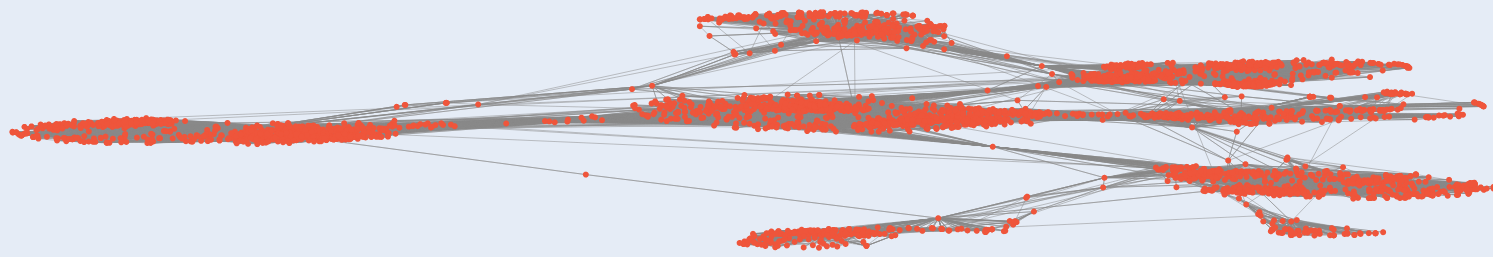
\includegraphics{./images/graph_facebook.png}
				}
				\caption{\small Projection 2D du graphe de Facebook}
				\end{figure}
			\end{column}
			\begin{column}[c]{0.5\textwidth}
				\begin{figure}
					\resizebox{\textwidth}{0.5\textheight}{
					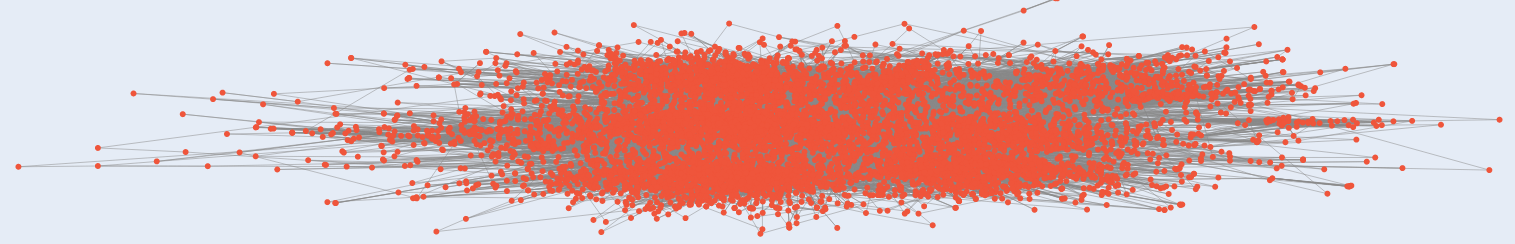
\includegraphics{./images/graph_lastfm.png}
				}
				\caption{\small Projection 2D du graphe de LastFM Asia}
				\end{figure}
			\end{column}
		\end{columns}
	\end{frame}

	\begin{frame}
		\frametitle{Visualisation de centralité}
		\begin{columns}
			\begin{column}[c]{0.5\textwidth}
				\begin{figure}
					\resizebox{\textwidth}{0.5\textheight}{
						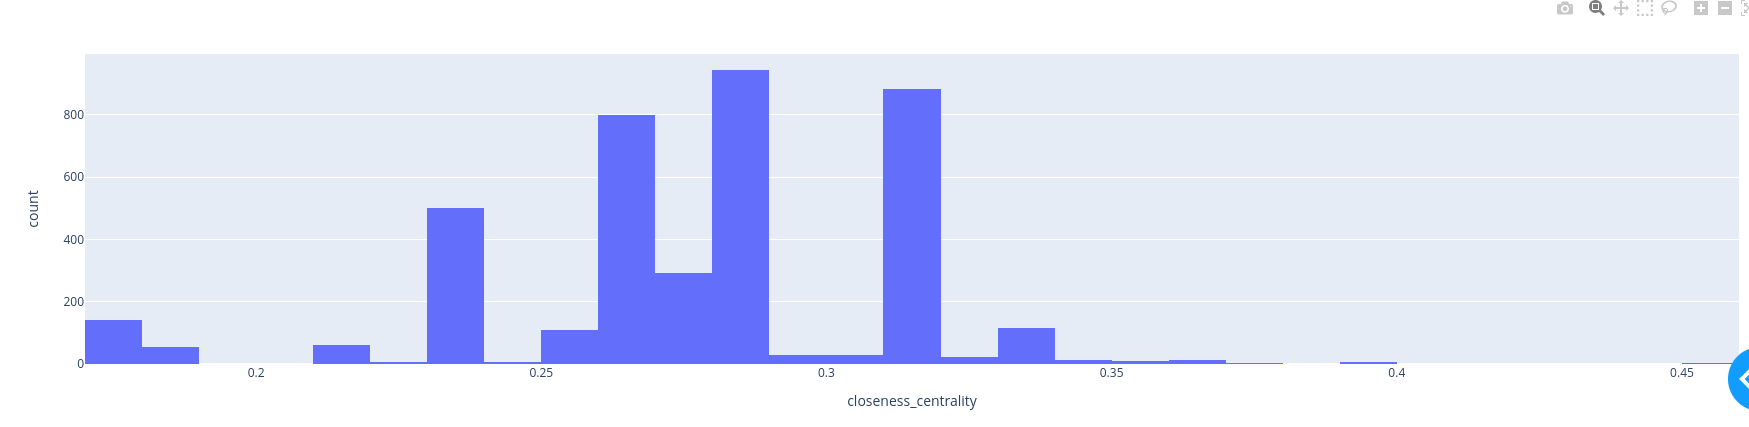
\includegraphics{./images/closeness_centrality_facebook.png}
					}
					\caption{\small Distribution de la centralité closeness sur le dataset de Facebook}
				\end{figure}
			\end{column}
			\begin{column}[c]{0.5\textwidth}
				\begin{figure}
					\resizebox{\textwidth}{0.5\textheight}{
						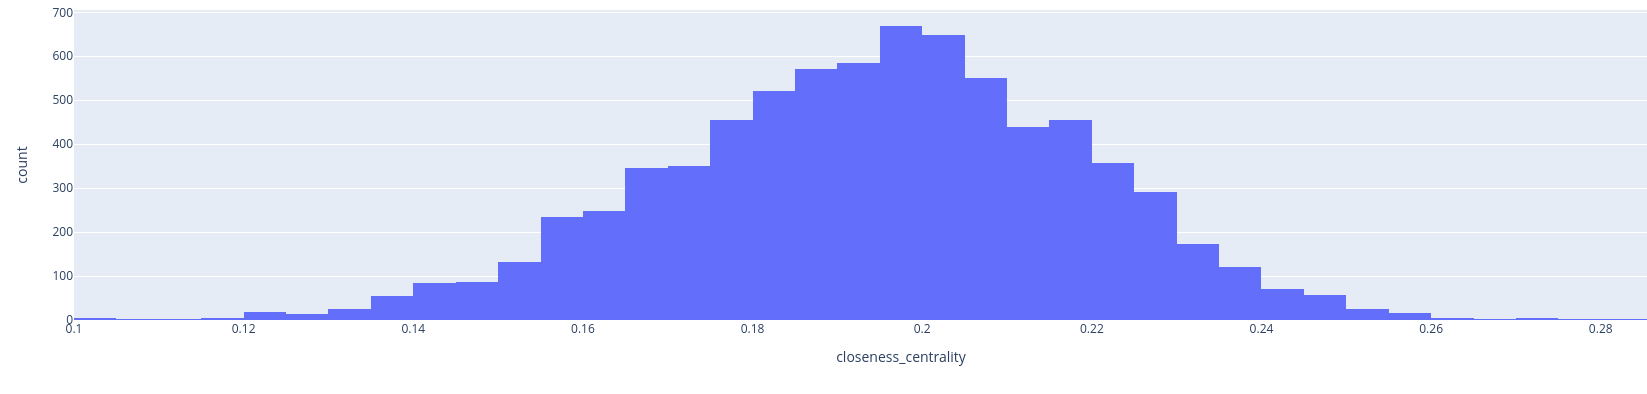
\includegraphics{./images/closeness_centrality_lastfm.png}
					}
					\caption{\small Distribution de la centralité closeness sur le dataset de LastFM Asia}
				\end{figure}
			\end{column}
		\end{columns}
	Sur les deux jeux de données, les autres centralités ont une distribution de type loi exponentielle.
	\end{frame}

	\begin{frame}
		\frametitle{Conclusion}
		
		\begin{itemize}
			\item La diffusion d'information sur les réseaux sociaux dépend de : 
		\begin{itemize}
			\item la stratégie de sélection des germes utilisée
			\item du modèle de diffusion
			\item de la topologie du réseau
		\end{itemize}
			\item Algorithmes de diffusion peuvent être coûteux en temps et en ressources même sur des petits réseaux
			\item Code du projet disponible sur github : \url{https://github.com/noblotni/graph_mining_labs}
		\end{itemize}
	
	\end{frame}
	
	
\end{document}